\section{Introduction}\label{sec:intro}
%Producing r
Reward is a fundamental signal that shapes our behavior through reinforcement learning (RL). 
Positive rewards encourage us to eat food and find mating partners, while negative rewards, such as pain and fatigue, help us protect ourselves. 
%Our brain produces a reward signal to a specific stimulus, such as good food, reinforcing our behavior to get more rewards. RL has been extensively studied in neuroscience and computer science. Neuroscientists have revealed that our brain has some hot or cold spots that respond to good or bad events~\citep{berridgeAffectiveNeurosciencePleasure2008}, and how those signals are used for learning~\citep{schultzNeuronalRewardDecision2015}, while computational reinforcement learning has provided theoretical models and several applications including game-playing agents and robotics~\citep{suttonReinforcementLearningIntroduction2018}.

% Problem: Reward evolution
% Why this topic has been underexplored, and how we can find some interesting points from this line of research
%In addition to RL, how the system for producing rewards has evolved is an interesting open question to understand our reward system. A common explanation is based on natural selection, arguing that 
Reward signals are supposed to have evolved to help animals survive and reproduce offspring (e.g., by~\cite{schultzNeuronalRewardDecision2015}), but how the variety or rewards, such as smells of foods or vision of s partners, 
evolved remains unclear.
%, although some neuroscientists guess external threat and the need of hunting could be infuential~\citep{ledouxSoonThereWas2022a}.

% Aim
This paper addresses this question from a computational perspective. 
Becase it is difficlt to observe the biological prosess of evolution of reward signals, we develop a simplified model of birth and death of RL agents in a 2D environment and examine what types of rewards evolve in a
% Why the population-based model is important
%For this purpose, we propose to use a population-based 
distributed evolution framework.
Previous studies on the evolution of learning \citep{hintonHowLearningCan1987,singhWhereRewardsCome2009} employed a centralized evolution scheme where all agents in the population are ranked and elites are selected as parents.
%While this approach is simple and computationally efficient, it sacrifices the biological reality. Instead, 
Our simulation model employs birth and death conditions depending on the energy level and the age. Each agent inherits a reward function from its parent and learns to get more rewards by RL during its lifetime. %Through this process, we expect that naturalistic reward functions will evolve.

We implement this framework using JAX\citep{jax2018git} to accelerate simulation by utilizing GPU. Our simulation results show that the evolution of food reward is surprisingly unstable due to the constraint of space and food resources.

\section{Preliminaries and Related Works}\label{sec:related}
We follow the standard computational RL framework \citep{suttonReinforcementLearningIntroduction2018} based on the Markov decision process (MDP). MDP $\M{}$ consists of a tuple $(\X{}, \A{}, p, r, \gamma)$, where $\X{}$ is state space, $\A{}$ is action space, $p: \X\times\A\times \X \rightarrow [0, 1]$ is state transition function, $r: \X\times\A \rightarrow \mathcal{R}$ is reward function, and $\gamma \in [0, 1]$ is the discount factor. A standard objective in MDP is the discounted cumulative return $G \defequal{} \sum_{t=0}^{\infty}\gamma^t R_{t}$, where $R_t$ is the reward received at time $t$. An RL agent has policy $\pi: \X \times \A \rightarrow [0, 1]$ and seeks to find the the optimal policy $\pi^{*}$ that maximizes $\E \left[G|\pi\right]$. The state-value function $V^\pi(s) \defequal \sum_{a \in \A} \pi(a|s) \left( r(s, a) + \gamma \sum_{s' \in \X} P(s'|s, a) V^\pi(s') \right)$ is often used in RL algorithms. Observation $o \in \Omega~(\Omega \subseteq \X)$ often refers to a part of the state that an agent can observe.

Our reward model is inspired by the neuroscience of reward system \citep{schultzNeuronalRewardDecision2015, berridgePleasureSystemsBrain2015}. Notably, \citet{berridgeDissectingComponentsReward2009} argue that the brain reward system consists of three independent components: liking, wanting, and learning. In analogy with computational RL, liking corresponds to reward function, wanting corresponds to learned policy, and learning corresponds to learning state value $V$. %\citet{dayanLikingEarlyEditable2022} discussed the idea that liking is related to reward shaping \citep{ngPolicyInvarianceReward1999} in computational RL that helps an agent to learn faster. This aligns with our view of rewards, although we don't focus on the quality of rewards in this paper.

While 
%we are focusing on the distributed evolution of rewards in a multi-agent setting, 
there were previous attempts to evolve rewards in a single-agent setting \citep{singhWhereRewardsCome2009,niekumEvolutionRewardFunctions2011,zhengWhatCanLearned2020},
%While evolutionary robotics studies \citep{nolfiEvolutionaryRoboticsBiology2004} often employ a centralized selection scheme similar to genetic algorithm \citep{mitchellIntroductionGeneticAlgorithms1998}, 
%where highly evaluated elites are selected as parents. On the contrary, 
we take a distributed embodied evolution (EE) framework \citep{watsonEmbodiedEvolutionDistributing2002,bredecheEmbodiedEvolutionCollective2018}
%that employs a decentralized evolution without centralized evaluation 
where agents evolve locally following birth and death rules. This method has an advantage that the evaluation of genetic traits depends population dynamics, which is more natural.

Our work is inspired by the series of studies \citep{elfwingBiologicallyInspiredEmbodied2005,elfwingDarwinianEmbodiedEvolution2011,elfwingEmergencePolymorphicMating2014}, which tried to evolve parameters related to RL through EE framework. Notably, \citet{elfwingDarwinianEmbodiedEvolution2011} evolved supplementary shapring rewards and parameters of RL agents.
%, and \citet{elfwingEmergencePolymorphicMating2014} evolved agents with a hierarchical RL mechanism, where the higher module chooses either foraging or mating, and the lower module outputs more primitive actions. 
Inspired by these works, we attempt to evolve all reward functions in this experiment.
%instead of hyperparameters.

%Among them, \citet{singhWhereRewardsCome2009} was pioneering in suggesting the idea that rewards should be internal to agents from the RL community.
\citet{zhengWhatCanLearned2020} was also inspiring to us in trying large-scale evolutionary simulation of rewards utilizing hardware accelerators.

\section{Simulation Model and Environment}\label{sec:method}

\begin{figure}[t]
  \centering{}
  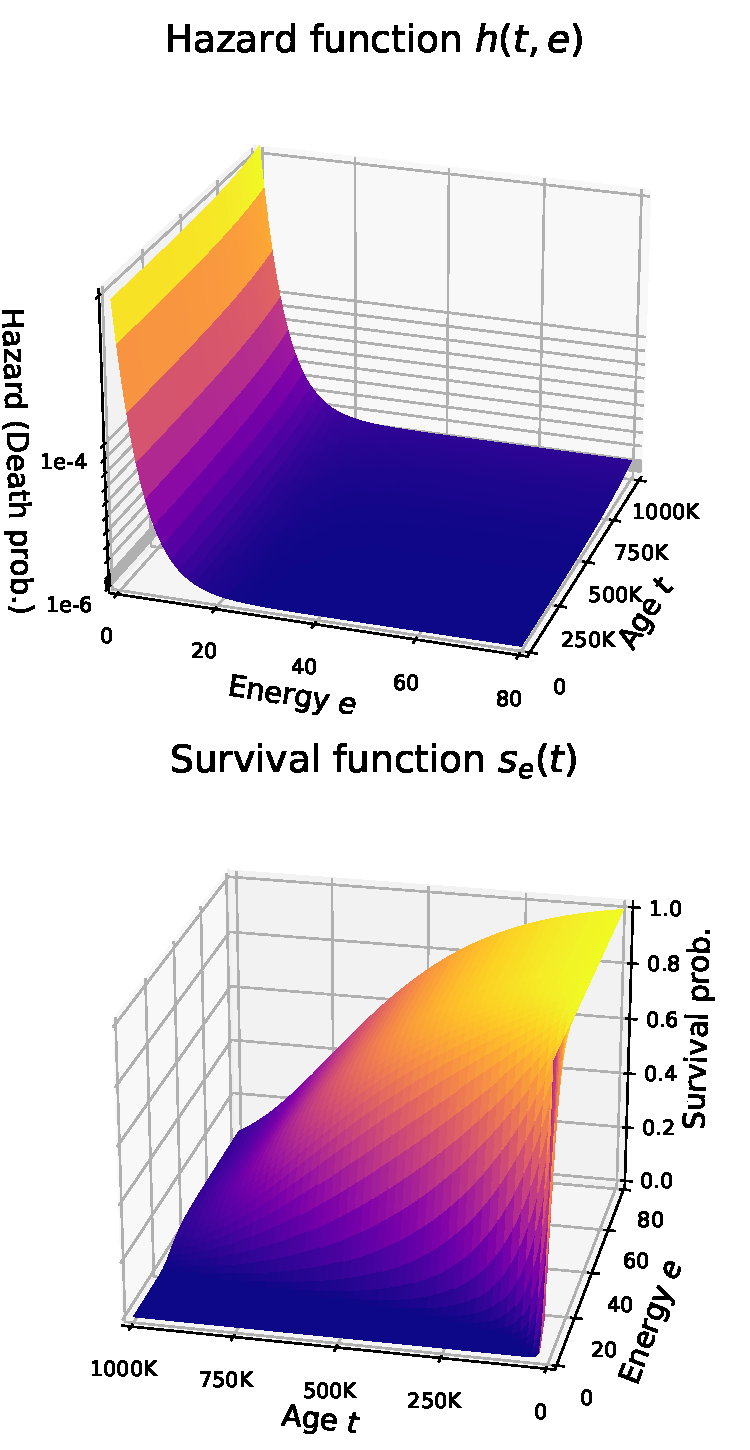
\includegraphics[width=15cm]{hazard_and_survival.pdf}
  \caption{
    \textbf{Left:} Designed hazard function $h(t)$ used for RL agents.
    \textbf{Right:} Survival function $S(t)$ corresponding to the hazard function.
  }\label{figure:hs}
\end{figure}

\paragraph{Energy-based death and birth model}
%As a simple but biologically plausible way of simulating the birth and death of agents, w
We employ an energy-based model similar to \citet{hamonEcoevolutionaryDynamicsNonepisodic2023}. Each agent maintains their energy level $e$, %Energy level $e$ 
which increases by eating a food and decreases by the basal metabolism and taking a motor action. 
We design the agent's death and birth model
%to maintain a higher energy level $e$, which leads to longer lives and many offspring. With 
based on $e$ and an agent's age $t$.
We adopt a Gompertz hazard model \citep{gompertzXXIVNatureFunction1825,kirkwoodDecipheringDeathCommentary2015}, in which the probability of an agent dying in a time step is given by:
\begin{align}
  h(t, e) = \frac{\kappa_{h}}{1 +  \exp(e - \theta_h)} + \alpha_{ht} \exp(\beta t). 
  % \theta_h = \log\alpha_{he}
  %h(t, e) = \kappa_{h} \left(1 - \frac{1}{1 + \alpha_{he} \exp(-e)} \right) + \alpha_{ht} \exp(\beta t). 
  \label{eq:h}
\end{align}

  %This hazard function\label{eq:h} consists of two terms. 
The first term increases as energy levels decrease and follow a sigmoidal curve, where $\kappa_{h}$ is the maximum death rate and $\theta_h$ is the energy threshold of increased death. %$\alpha_{he}$ are hyperparameters. 
The latter term %$\alpha_{ht} \exp(\beta t)$ 
exponentially increases as the agent gets older.
%, where $\alpha_{ht}$ and $\beta$ are hyperparameters. 
%In population statistics, this is called the Gompertz hazard model \citep{gompertzXXIVNatureFunction1825,kirkwoodDecipheringDeathCommentary2015}. 
The left panel in \Cref{figure:hs} shows the shape of the hazard function with the specific parameters used in our experiments. 
%To intuitively understand the behavior $h$, we plot 
The right panel in \Cref{figure:hs} shows the
survival function $S(t, e) = \exp (-\int_{0}^{t}(h(t, e)) dt)$, the probability for an agent to survive to the age $t$ if it keeps the same energy level $e$. 
We can see that the survival probability more sharply decays with aging when the energy level is low.

\begin{figure}[t]
  \centering{}
  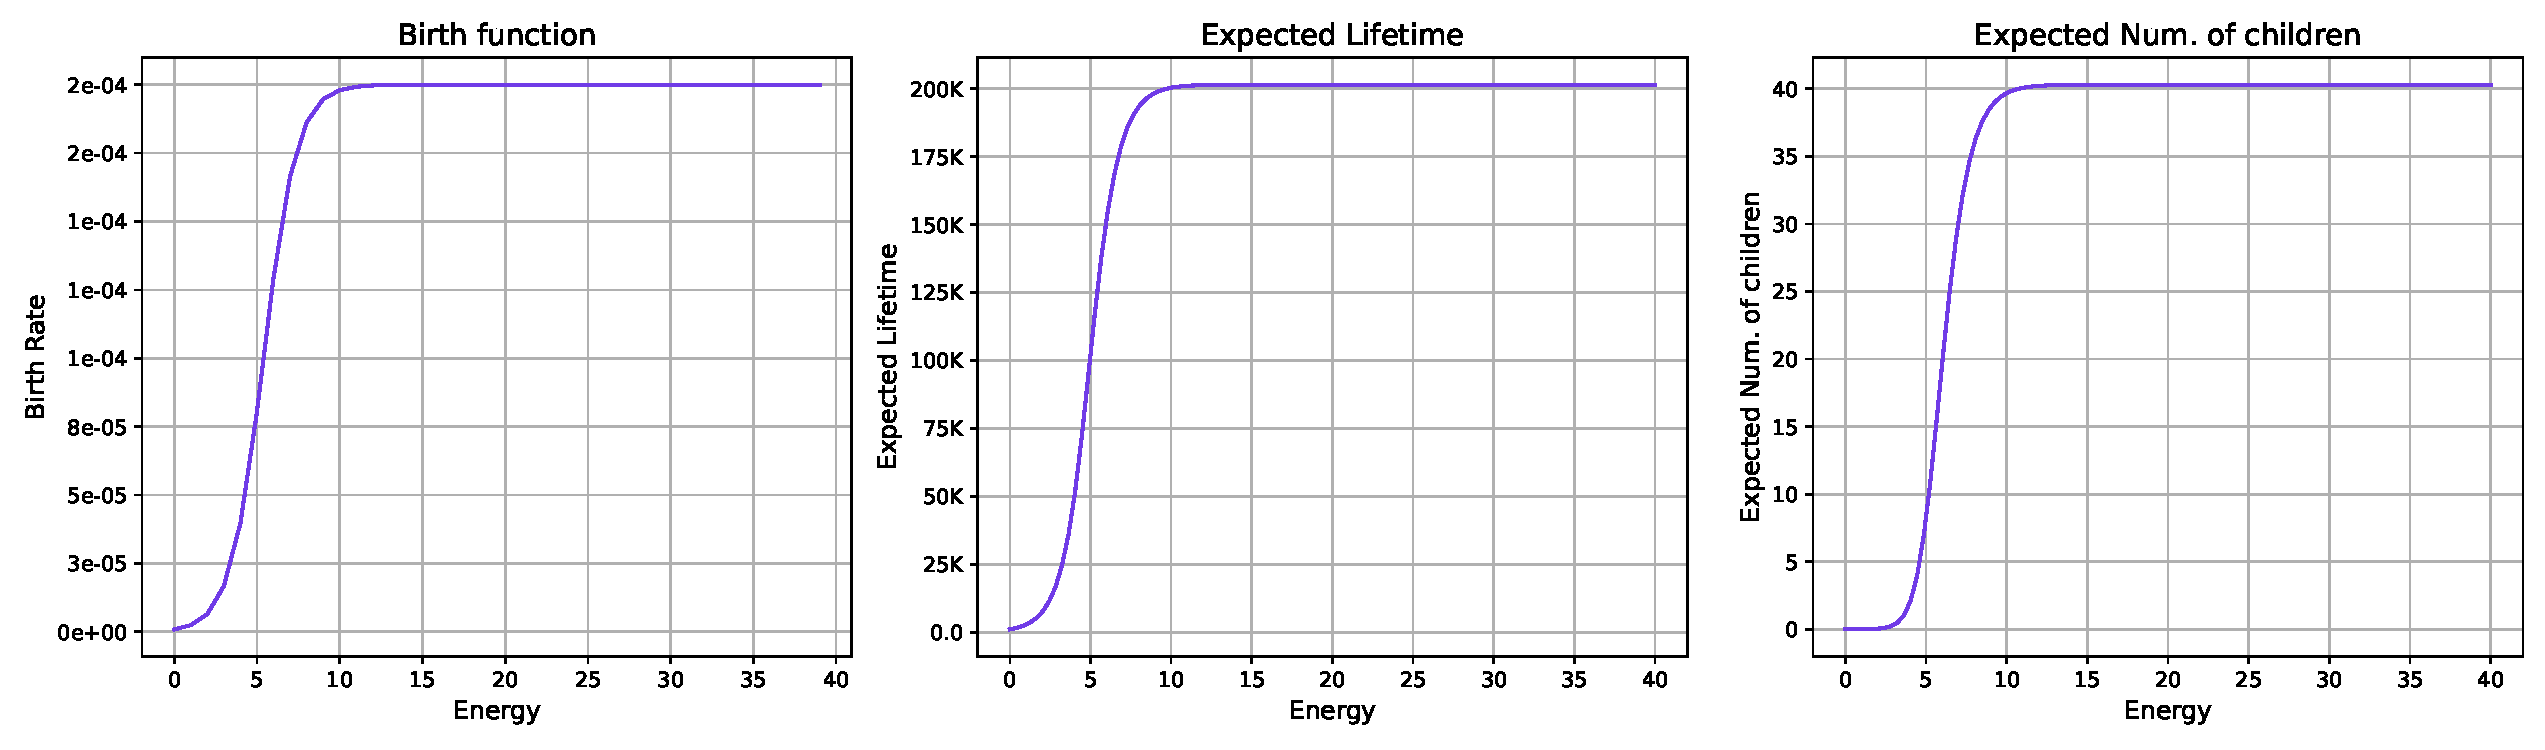
\includegraphics[width=15cm]{birth_and_nc.pdf}
  \caption{
    The left figure shows the designed birth rate $b(e)$ for RL agents, the center figure shows the expected lifetime for each agent, and the right figure shows the expected reproduction number $R$ for RL agents corresponding to the designed hazard and birth functions.
  }\label{figure:bnc}
\end{figure}

For simplicity, we employ an asexual reproduction model 
%where all agents can have a chance to make their children. We let $b(e)$ the birth function that evaluates the probability for an agent with energy level $e$ to make its child. Similarly to the first term of \cref{eq:h}, we design 
with the birth function, the probability for an agent with energy level $e$ to produce a child in a time step as:
\begin{align}
 b(e) &= \frac{\kappa_{b}}{1 + \alpha_{b}\exp(\theta_{b} - e)}. 
 % This parameterizaiton is redundant:
 % \alpha_{b}\exp(\theta_{b} - e)} = \exp(\log\alpha_{b} + \theta_{b} - e)}
 % It is more reasonable to use \beta_e inside \exp() to control the slope...
 \label{eq:b}
\end{align}
%Modeled as a generalized logistic function \citep{richardsFlexibleGrowthFunction1959}, 
The birth rate $b(e)$ increases with $e$ following a sigmoidal curve where $\kappa_{b}$ is the scale, $\theta_{b}$ controls the threshold of reaction, and $\alpha_{e}$ defines the shape of when $e = \theta_{b}$. 
The left figure of \Cref{figure:bnc} shows the shape of $b$ for the parameters used in the experiment. 
Based on the birth model $b(e)$ and the death model $h(e,t)$, we plot the expected lifetime and number of children if an agent keeps the same energy level in the center and right figure in \cref{figure:bnc}. Parameters are chosen so that the maximum expected lifetime is around \num{200000} and the maximum expected number of children is around 40. All experiment parameters are shown in \cref{ap:param}.

\paragraph{Environment}

\begin{figure}[t]
  \begin{subfigure}[t]{6cm}
    \centering
    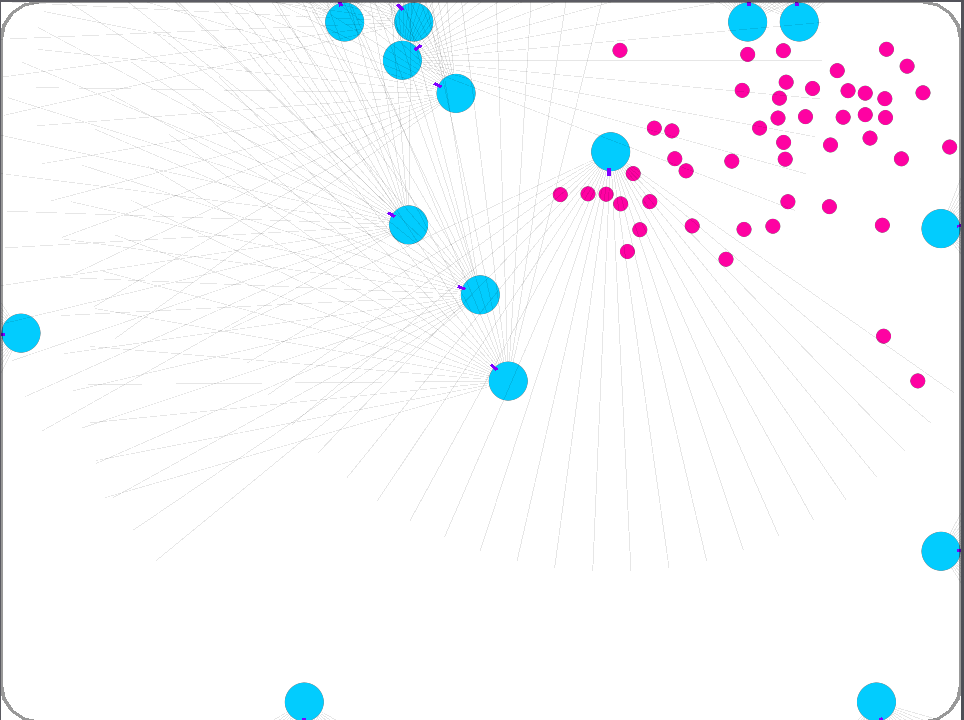
\includegraphics[width=6cm]{emevo-ss.png}
    \subcaption{Simulation environment we used in our experiments.}
  \end{subfigure}
  \begin{subfigure}[t]{8cm}
    \centering
    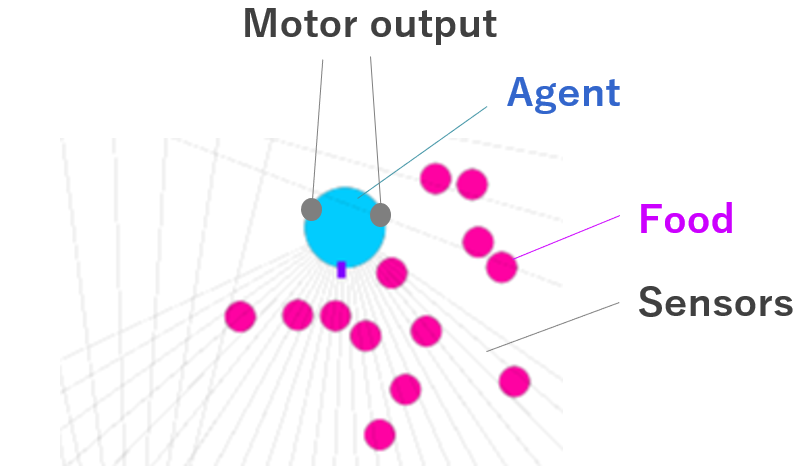
\includegraphics[width=8cm]{emevo-anno.png}
    \subcaption{Description of the environment}
  \end{subfigure}
  \caption{
    In the right figure, thin gray lines around agents indicate distance that can detect the distance to the closest object. Red circles indicate food. Outer gray lines are walls.
    In the right figure, An agent can move by adding force to two indicated points.
  }\label{figure:env}
\end{figure}

%As a simple simulation environment with biologically plausible sensorimotor interaction, w
We designed a continuous 2D environment shown in \Cref{figure:env}. Blue circles indicate agents and red circles indicate foods. The environment is implemented by a 2D rigid-body physics simulation, where agents can move by 
%adding motor outputs 
producing driving forces on the left and right sides of the body.
%at two points in the diagonal back part of the circle. 
%We use these two motor outputs as an action of agent in RL. 
An agent has multiple range sensors in its front, which can sense the type and the distance to the closest object (food, agent, and wall) within a certain range 
%and closest among three. We explain the details in 
(see \cref{ap:env}).

An agent can eat food by touching it and gain energy $e_{\mathrm{food}}$. After foods are eaten, they are regenerated in a random place.
% This eat-driven emergence is not consistent with the growth model below. Better report the actual food producing process rather than theoretical approximation.
%The rate of food regeneration follows logistic growth function $\frac{dN_{food}}{dt} = g N_{food} (1 - \frac{N_{food}}{N_{food}^{\mathrm{max}}}$, where $N_{food}$ is the number of food, $g$ is growth rate, and $N_{food}^{\mathrm{max}}$ is the maximum number of food. 
Eating food increases an agent's internal energy by $e_{\mathrm{food}}$. In some experiments, we use poisonous food that decreases energy level by $e_{\mathrm{poison}}$.

When an agent makes a child, a new agent is placed in a random location sampled from a Gaussian distribution centered around its parent. %However, to speed up the simulation, r
Reproduction fails when all
% report how many times.
sampled locations are not available. Thus, keeping away from the wall and other agents is beneficial for agents in order to make more children. When a child is produced
%the parent's energy level is $e$, 
a proportion of the parent's energy $\eta e \in [0, 1]$ is given to the child and the parent's energy level decreases to $(1-\eta)e$.
%, where $\eta \in [0, 1]$ is the ratio of energy sharing. 
The child also inherits its reward function from the parent with some mutation.

%Simulating many agents to maintain a reasonable size population (e.g., $50\sim 100$) is key in our evolution scheme. 
To speed up the simulation, we implement our environment using JAX Python library \citep{jax2018github} to utilize GPU or other hardware accelerators. Inspired by recent works on 3D rigid body physics simulation using JAX (e.g., \citet{brax2021github} and MuJoCo \citep{todorov2012mujoco} MJX\footnote{\url{https://mujoco.readthedocs.io/en/stable/mjx.html}}), we implement our 2D physics engine using JAX and build our environment on top of that, optimizing it for multi-agent setting. We explain the implementation detail in \cref{ap:phys}.

\paragraph{Reward Function with Evolving Weights} %Parameters}
We assume that the reward function is detemined at birth with mutation and does not changed during an agent's lifetime. As inputs to the reward function, we consider \rnum{1} collision to food (eating), \rnum{2} collision to the wall, \rnum{3} collision to some other agent, and \rnum{4} the magnitude of agent's action (motor output). In experiments with poisonous food, the collision with food is also included. 
We expect that positive reward for food evolves to acquire energy
and negative reward for action  evolves to save energy. Collisions with the wall and other agents are chosen to test if the reward function can distinguish unrelevant signals for survival, as we do not penalize agents for colliding with walls or each other.

We take a linear model the reward function with weights for each sensory input
\begin{align}
  r = \sum_i r_i = \sum_i w_i f_i
  \label{eq:reward}
\end{align}
where $w_i$ is the weight for a sensorimotor event $f_i$ for $i\in{\mbox{\{foood, wall, agent,  action\}}}$.
% This redundant coding is better put to Appendix
%For example, the reward weight for getting food is modeled as $r_{\mathrm{food}} = 10^{s_{\mathrm{food}}} w_{\mathrm{food}}$, where $s_{\mathrm{food}} \in [0, 1]$ and $w_{\mathrm{food}} \in [-1, 1]$ are evolvable parameters that represent scale and weight for the food reward weight. 
%We model reward weights for other sensory inputs by $r_\mathrm{wall}$, $r_\mathrm{agent}$, and $r_\mathrm{agent}$ in the same way. 
%Our intention in using two independent parameters $s$ and $w$ is to balance stability and plasticity. Our preliminary experiments found that rewards can be too unstable if we allow significant change via a single parameter. Having a parameter for adjusting the scale separately makes the significant reward change more challenging while still possible. Reward weights are multiplied by collision events or action magnitude and then summed up to the reward that an agent uses in RL. 
We explain the detail of implementation in \cref{ap:reward}.

% Add a line for reward acquisition; after observation or action?
\begin{algorithm}
  \caption{Reward evolution with asexual reproduction}\label{alg:reward-evo}
  \begin{tabular}{lll}
    \textbf{Input:} & $Pop, Env$ & Initial population and simulation environment\\
                    & $N$ & Number of rollout steps used in RL \\
                    & $h(t, e)$, $b(e)$ & Hazard and birth function for agents \\
                    & $mut(r)$ & Mutation function for reward function \\
                    & $\eta$ & Energy share ratio used in reproduction
  \end{tabular}
  \begin{algorithmic}[1]
    \Loop{}
    \ForAll{$agent \in Pop$}
      \State{$o \gets agent$'s observation in $Env$}
      \State{Sample an action $a$ from $agent$'s policy $\pi_{agent}(\cdot|o)$}
      \State{Update $agent$'s energy level $e$ based on the taken action $a$ and eaten food}
      \Once{in $N$ steps}
        \State{Update $agent$'s policy $\pi_{agent}$ and value function $\vh_{agent}$ via RL}
      \EndOnce{}
    \EndFor{}

    \State{Step the simulated environment $Env$ one step using collected actions}
    \LComment{Process death and birth}
    \ForAll{$agent \in Pop$ with energy level $e$, age $t$, and reward function $r$}
      \With{Probability $b(e)$}
        \State{$e_\mathrm{new} \gets \eta e$, $r_\mathrm{new} \gets mut(r)$}
        \State{Add a new agent with reward function $r_\mathrm{new}$ and energy level $e_\mathrm{new}$ to $Pop$ and $Env$}
        \State{Update parent's energy to $(1 - \eta) e$}
      \EndWith{}
      \With{Probability $h(t, e)$}
        \State{$agent$ is removed from $Pop$ and $Env$}
        \Comment{agent is dead}
      \EndWith{}
    \EndFor{}
  \EndLoop{}
\end{algorithmic}
\end{algorithm}

\paragraph{Simulation Procedure}
We show the pseudocode of our entire simulation procedure in \cref{alg:reward-evo}. Each agent has its innate, immutable reward function and learnable neural network policy. At each step, it observes sensory inputs from the environment and takes action. Once in $N$ steps, the agent updates its policy via RL using the past $N$ step experiences. We use Proximal Policy Optimization \citep{schulmanProximalPolicyOptimization2017} as an RL algorithm because of its fast computation time. We explain the details of our RL implementation in appendix \todo{Write appendix}. After environmental interaction, all agents can make a child and die based on the birth function $b$ and hazard function $h$. The new agent inherits a fraction of the parent's energy and mutated reward function. As mutation, we add uniform noise to each $s$ and $w$ with probability $0.4$. We show some relevant parameters in \cref{ap:param}.

\section{Results}

\begin{figure}[t]
  \begin{subfigure}[t]{7.5cm}
    \centering
    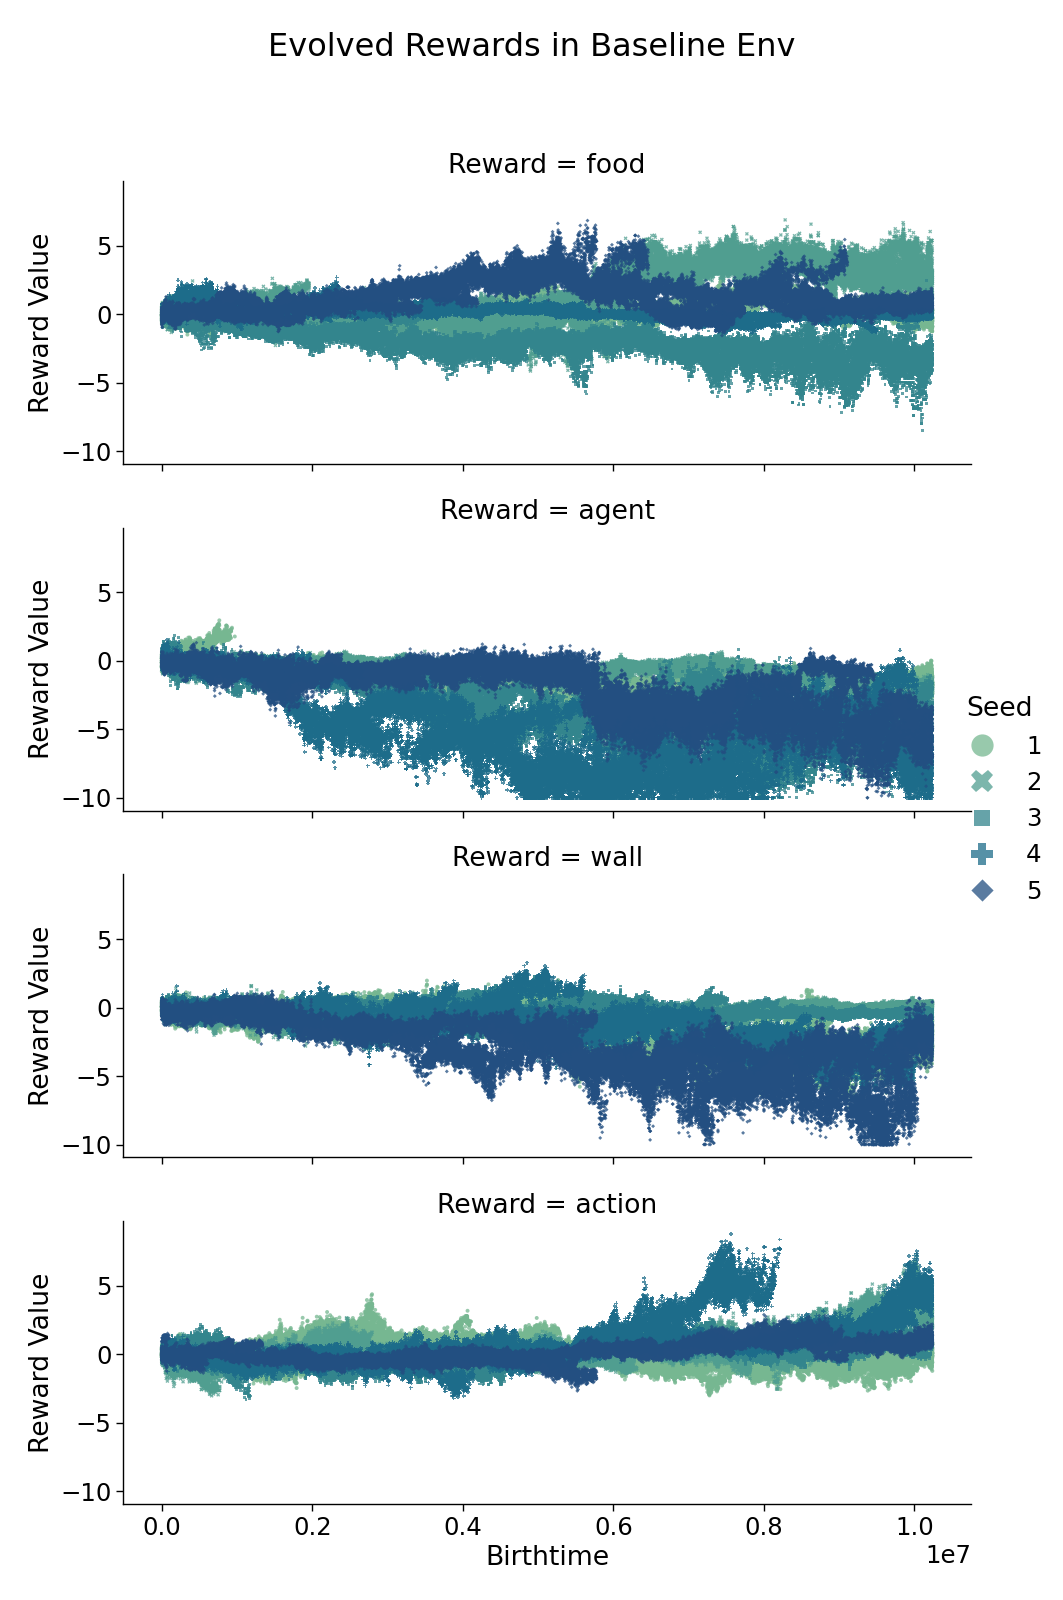
\includegraphics[width=7.5cm]{baseline.png}
    \subcaption{Evolved rewards in the baseline environment.}\label{subfigure:bl}
  \end{subfigure}
  \begin{subfigure}[t]{7.5cm}
    \centering
    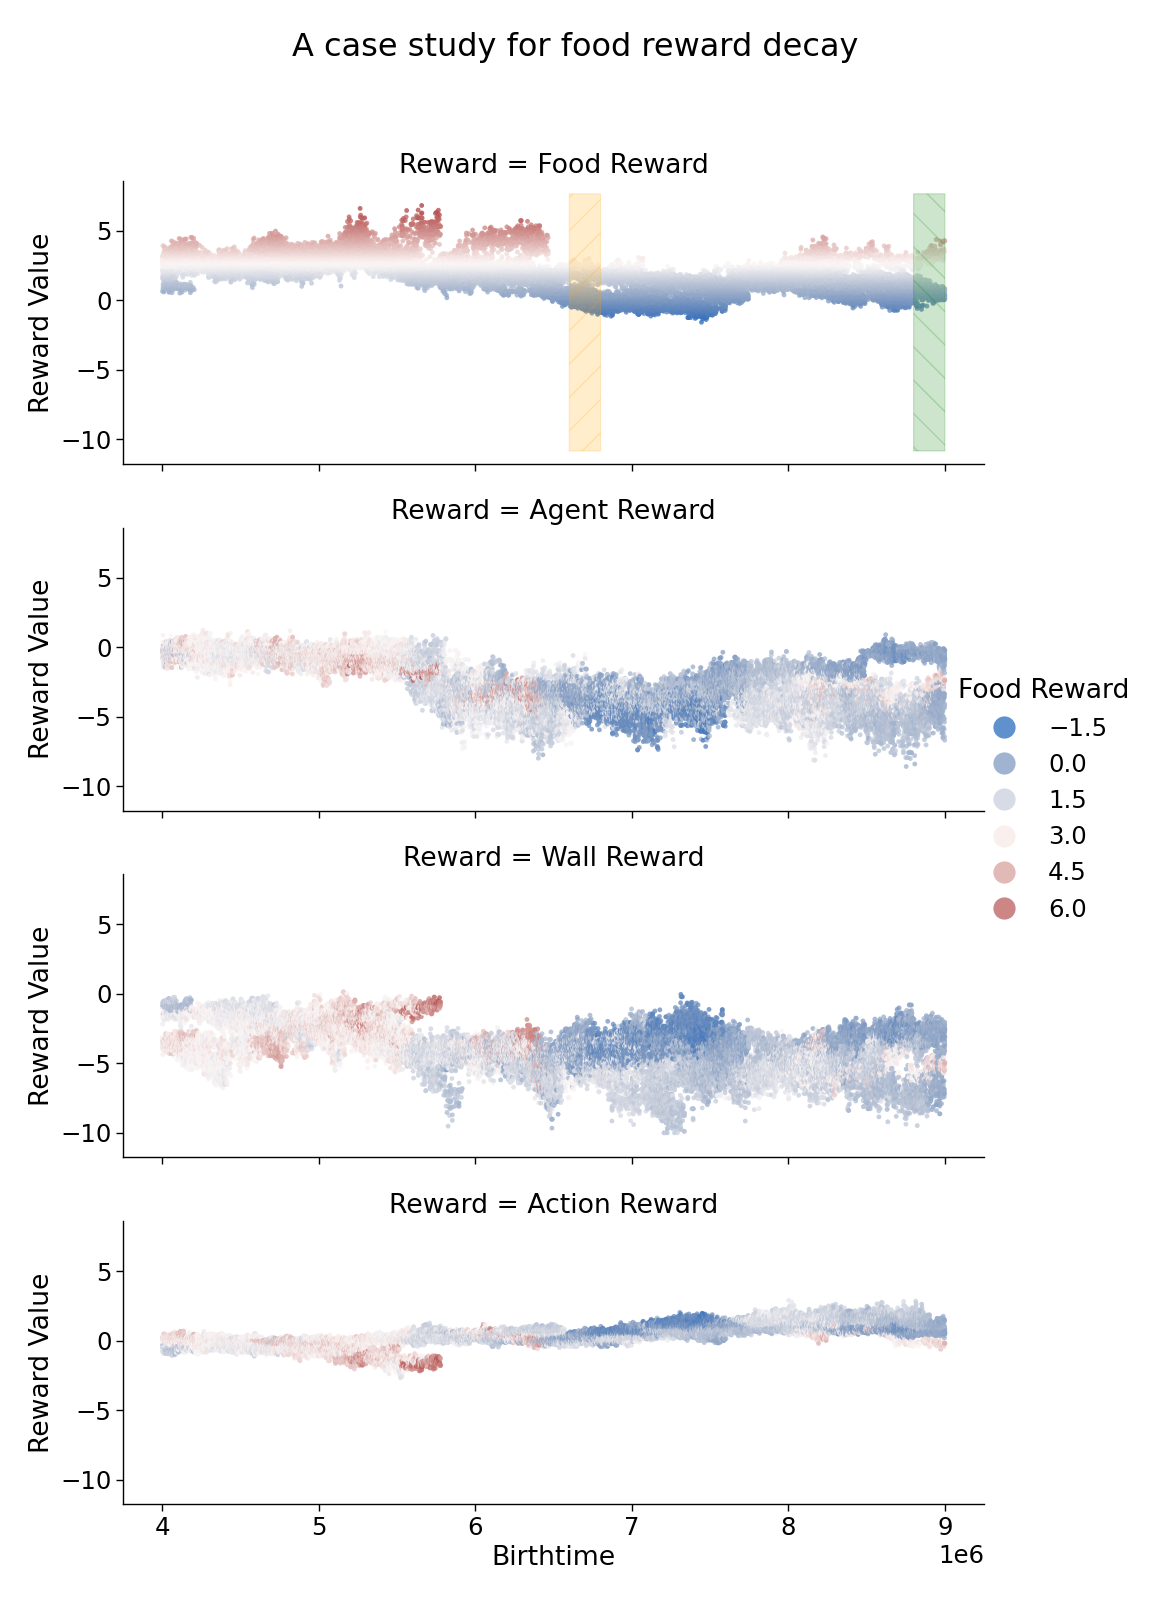
\includegraphics[width=7.5cm]{seed5-frdecay.png}
    \subcaption{A case study for decreasing food reward.}\label{subfigure:s5cs}
  \end{subfigure}
  \caption{
    In the left figure, the X-axis shows the birth time of each agent, and the y-axis shows the value of rewards for food, agent, wall, and action from top to bottom. The difference in colors and shapes of dots corresponds to the difference in the random seed. The right figure colarized the reward weights per food reward in case the food reward decreases. We selected the run with seed $5$ from \num{4e6} to \num{9e6} steps for this purpose.
  }\label{figure:baseline-result}
\end{figure}

As a baseline environment, we use the setting where food is always regenerated in the upper right of the room, as the left figure in \Cref{figure:env} shows. In this environment, we tuned environmental parameters (e.g., maximum number of foods and growth rate) to stabilize the population around $100$. We show all environmental parameters in \cref{ap:param}. All experiments start with $50$ agents that have energy level $40.0$ and randomly initialized reward weights. We conducted \num{1e7} step of the simulation, resulting in 10 \todo{actual number} generations, which takes $14\sim16$ hours on NVIDIA P100 GPUs.

\Cref{subfigure:bl} shows the evolved reward weights with 5 random seeds in the baseline environment. Surprisingly, the food reward weight is only stable positive for one random seed. It unstably goes up and down or stays negative in one random seed. On the contrary, reward weights for colliding with walls and other agents are stably negative, which is reasonable because sticking around walls is not good for foraging, and sticking to other agents might reduce the chance of making a child. The reward weight for action tends to be positive. This contradicts our expectations that it would evolve to negative like fatigue.

\begin{figure}[t]
  \begin{subfigure}[t]{7cm}
    \centering
    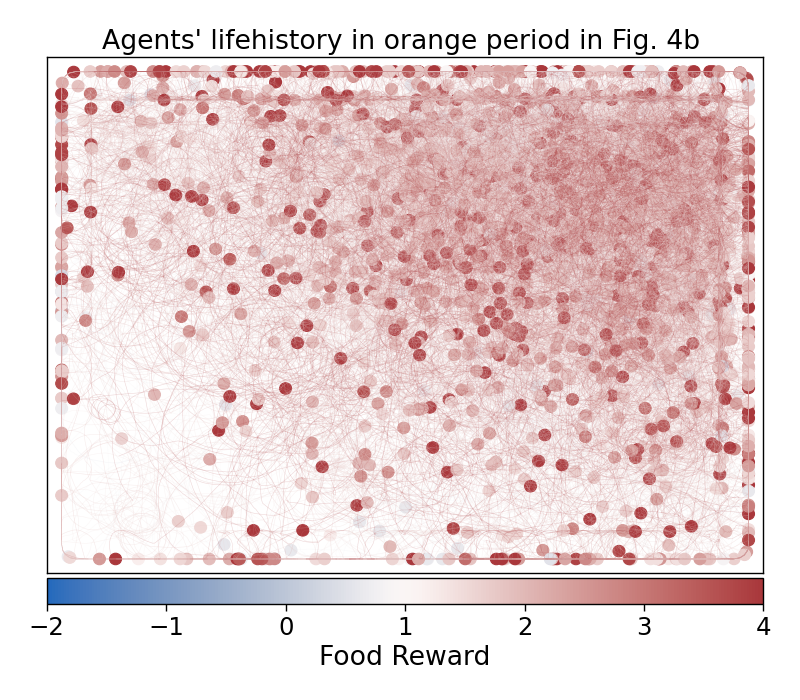
\includegraphics[width=7cm]{seed5-lh-orange.png}
  \end{subfigure}
  \begin{subfigure}[t]{7cm}
    \centering
    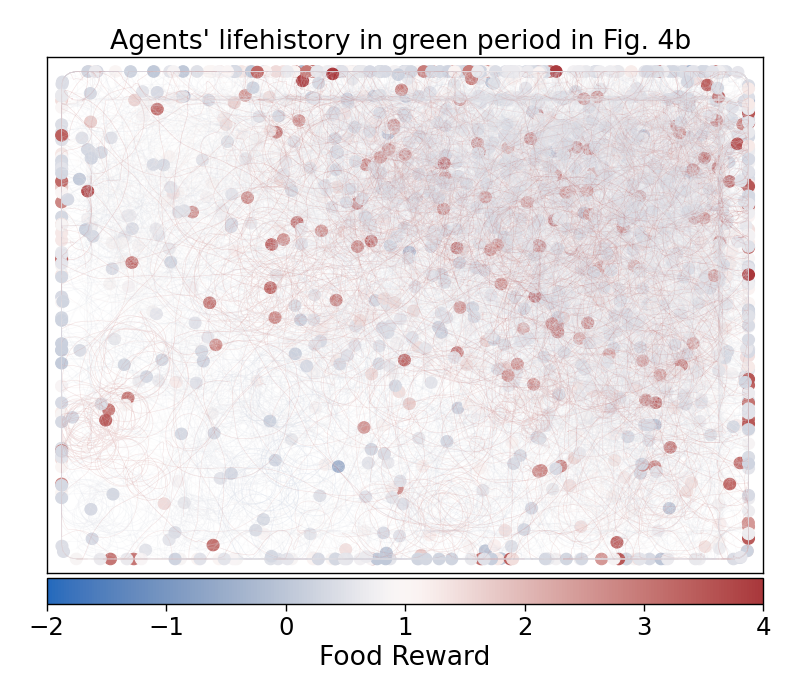
\includegraphics[width=7cm]{seed5-lh-green.png}
  \end{subfigure}
  \caption{
    Agent's life history corresponding to \cref{subfigure:s5cs}. The left figure corresponds to the period filled with orange and \texttt{/}, and the right figure corresponds to the period filled with green and \texttt{\textbackslash}. Lines show trajectories of agents, colored by their food reward weight. Dots show places where agents made a child.
  }\label{figure:s5-lh}
\end{figure}

To investigate the reason why the evolution of food reward can be unstable, we closely look at our simulation run with seed $5$, where food reward decreases. \Cref{subfigure:s5cs} shows the scatter plot of reward weights in this run from \num{4e6} to \num{9e6} steps, where blue color indicates smaller food rewards and red color indicates larger. We can see a tendency that agents with lower food rewards tend to have higher wall and action rewards, which is reasonable because both sticking around walls and just moving can help foraging. On the contrary, we can see two different modes in agent and action rewards. In the medium of \cref{subfigure:s5cs} (between \num{6e6} and \num{7e6} steps), agents with smaller rewards tend to have smaller negative rewards for colliding with agent, while they tend to have larger agent rewards later. To investigate the reason why food reward decreases more, we focus on the period we filled orange and green in the first row of \cref{subfigure:s5cs}, where both negative and positive food rewards coexist. We plot life history of agents in these period in \cref{figure:s5-lh}, where thin lines show the agents' trajectories, dots show places where agents got child, and different colors corresponds to the value of food rewards. In both figures, we can see that agents trajectories are concentrated around the food location, but places where agents got child are more distributed because of the environmental constraint that it's difficult to make a child in a crowded area. Here, we don't see significant differences in trajectory or birth location in either case. In the figure on the left, the locations where agents with high food rewards gave birth are often a bit distant from the top right corner of the figure where the food is located. We suspect that this is because the food location is too crowded, and this is the reason why large negative agent reward started to evolve in this situation. Keeping distance from another agents is beneficial to get more opportunity to get children. Interestingly, we can't see this tendency in the right figure, because overconcentration of populations is suppressed by agents with negative food rewards, although they still tend to gather around the food location thanks to the positive rewards for colliding with another agent.

%   \textbf{Right:} Evolved rewards in multiple settings, including the baseline environment. Each line shows the reward weight averaged over all agents alive at that time. Different colors indicate different settings.

\section{Conclusion}